\documentclass{book}
\usepackage{import}
\import{//home/vatican/officium-simplex/modules/}{def-packages}
\import{//home/vatican/officium-simplex/modules/}{def-macros}
\import{//home/vatican/officium-simplex/modules/}{def-pages}
\geometry{a5paper,hdivide={1cm,*,1cm},vdivide={1cm,*,1cm}}
\begin{document}
\begin{center}
    \LARGE Arquidiocese de Olinda e Recife
    \vspace{.1cm} \\
    \LARGE Vicariato Paulista
    \vspace{.1cm} \\
    \LARGE Comissão Pastoral para a Liturgia
    \vspace{.2cm} \\
    \textcolor{VioletRed2}{\Large Retiro dos candidatos ao ministério extraordinário da sagrada comunhão eucarística}
    \vspace{.4cm} \\
    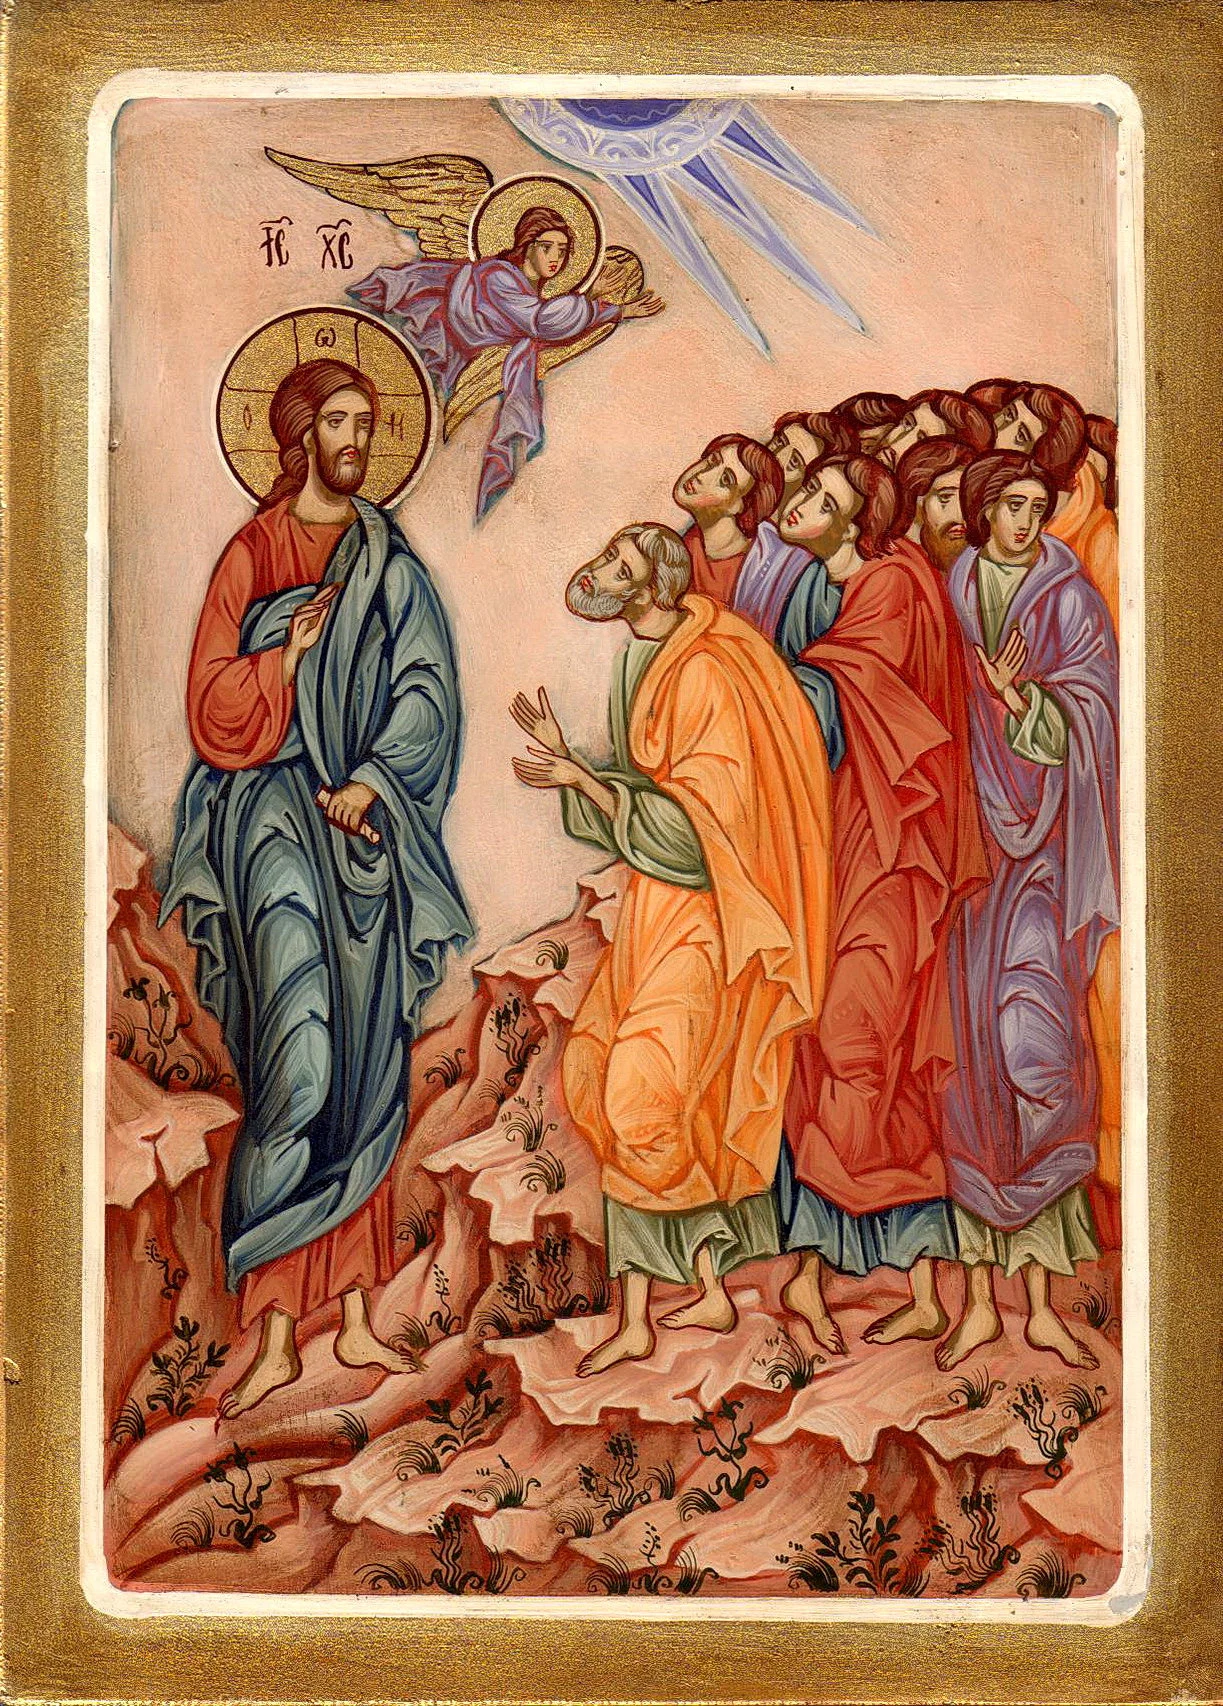
\includegraphics[scale=0.2]{/home/vatican/officium-simplex/src/Jesus.jpg}
    \vspace{.4cm} \\
    \textcolor{VioletRed2}{\Large 21\textordmasculine{} Domingo do Tempo Comum}
    \vspace{\fill}\\
    \Large Paulista, 25 de Agosto de 2024
\end{center}

\newpage
\begin{center}
    \textbf{Oração Inicial}
    \vspace{.2cm} \\
    \textcolor{VioletRed2}{\textbf{21\textordmasculine{} Domingo do Tempo Comum}}
    \vspace{.2cm} \\
    \textbf{Laudes}
    \vspace{.2cm} \\
    \VbarRed{} Vinde, ó Deus, em meu auxílio. \\
    \RbarRed{} Socorrei-me sem demora. \\
    Glória ao Pai e ao Filho e ao Espírito Santo.\ \textsuperscript{\gresixstar{}} \\
    Como era no princípio, agora e sempre, Amém. Aleluia.
    \vspace{.2cm} \\
    \textcolor{VioletRed2}{Hino}
    \vspace{.2cm} \\
    Ó Criador do universo, \\
    a sombra e a luz alternais, \\
    e, dando tempo ao tempo, \\
    dos seres todos cuidais.
    \vspace{.2cm} \\
    Qual pregoeiro do dia, \\
    canta nas noites o galo. \\
    Separa a noite e a noite, \\
    brilhando a luz no intervalo.
    \vspace{.2cm} \\
    Também por ele acordada, \\
    a estrela d'alva, brilhante, \\
    expulsa o erro e a treva \\
    com sua luz radiante.
    \vspace{.2cm} \\
    Seu canto os mares acalma, \\
    ao navegante avigora; \\
    a própria Pedra da Igreja \\
    ouvindo o cântico chora.
    \vspace{.2cm} \\
    Jesus, olhai os que tombam. \\
    O vosso olhar nos redime: \\
    se nos olhais, nos erguemos, \\
    e prantos lavam o crime.
    \vspace{.2cm} \\
    Ó luz divina, brilhai, \\
    tirai do sono o torpor. \\
    O nosso alento primeiro \\
    entoe o vosso louvor.
    \vspace{.2cm} \\
    Ó Cristo, Rei piedoso, \\
    a vós e ao Pai, Sumo Bem, \\
    glória e poder, na unidade \\
    do Espírito Santo. Amém.
    \newpage
    \textcolor{VioletRed2}{Salmodia}
    \vspace{.2cm} \\
    \textcolor{VioletRed2}{Ant.} Desde a aurora ansioso vos busco, \\
    para ver vossa glória e poder.
    \vspace{.2cm} \\
    \textcolor{VioletRed2}{Salmo 62(63),2-9}
    \vspace{.2cm} \\
    \textbf{Sede de Deus} \\
    \textit{Vigia diante de Deus, quem rejeita as obras das trevas (cf. 1Ts 5,5).}
    \vspace{.2cm} \\
    \textsuperscript{\underline{\hspace{.06in}}\textcolor{VioletRed2}{2}}Sois vós, ó Senhor, o meu Deus! \textsuperscript{\gresixstar{}} \\
    Desde a aurora ansioso vos busco! \\
    = A minh'alma tem sede de vós, \dag{} \\
    minha carne também vos deseja, \textsuperscript{\gresixstar{}} \\
    como terra sedenta e sem água!
    \vspace{.2cm} \\
    \textsuperscript{\underline{\hspace{.06in}}\textcolor{VioletRed2}{3}}Venho, assim, contemplar-vos no templo, \textsuperscript{\gresixstar{}} \\
    para ver vossa glória e poder. \\
    \textsuperscript{\underline{\hspace{.06in}}\textcolor{VioletRed2}{4}}Vosso amor vale mais do que a vida: \textsuperscript{\gresixstar{}} \\
    e por isso meus lábios vos louvam.
    \vspace{.2cm} \\
    \textsuperscript{\underline{\hspace{.06in}}\textcolor{VioletRed2}{5}}Quero, pois, vos louvar pela vida, \textsuperscript{\gresixstar{}} \\
    e elevar para vós minhas mãos! \\
    \textsuperscript{\underline{\hspace{.06in}}\textcolor{VioletRed2}{6}}A minh'alma será saciada, \textsuperscript{\gresixstar{}} \\
    como em grande banquete de festa; \\
    \textsuperscript{\underline{\hspace{.06in}}} Cantará a alegria em meus lábios, \textsuperscript{\gresixstar{}} \\
    ao cantar para vós meu louvor!
    \vspace{.2cm} \\
    \textsuperscript{\underline{\hspace{.06in}}\textcolor{VioletRed2}{7}}Penso em vós no meu leito, de noite, \\
    nas vigílias suspiro por vós! \\
    \textsuperscript{\underline{\hspace{.06in}}\textcolor{VioletRed2}{8}}Para mim fostes sempre um socorro; \textsuperscript{\gresixstar{}} \\
    de vossas asas à sombra eu exulto! \\
    \textsuperscript{\underline{\hspace{.06in}}\textcolor{VioletRed2}{9}}Minha alma se agarra em vós; \textsuperscript{\gresixstar{}} \\
    com poder vossa mão me sustenta.
    \vspace{.2cm} \\
    \textsuperscript{\underline{\hspace{.06in}}} Glória ao Pai e ao Filho e ao Espírito Santo.\ \textsuperscript{\gresixstar{}} \\
    Como era no princípio, agora e sempre. Amém.
    \vspace{.2cm} \\
    \textcolor{VioletRed2}{Ant.} Desde a aurora ansioso vos busco, \\
    para ver vossa glória e poder.
    \vspace{.2cm} \\
    \textcolor{VioletRed2}{Leitura breve Ap 7,10b-12}
    \vspace{.2cm} \\
    A salvação pertence ao nosso Deus, que está sentado no trono, e ao Cordeiro. O louvor, a glória e a sabedoria, a ação de graças, a honra, o poder e a força pertencem ao nosso Deus para sempre. Amém.
    \newpage
    \textcolor{VioletRed2}{Cântico evangélico (Benedictus) \\ Lc 1,68-79}
    \vspace{.2cm} \\
    \textcolor{VioletRed2}{Ant.} Ninguém poderá vir a mim, \\
    se pelo Pai não lhe for concedido.
    \vspace{.2cm} \\
    \textbf{O Messias e seu Precursor}
    \vspace{.2cm} \\
    \textsuperscript{\underline{\hspace{.06in}}\textcolor{VioletRed2}{68}}Bendito seja o Senhor Deus de Israel, \textsuperscript{\gresixstar{}} \\
    porque a seu povo visitou e libertou;
    \vspace{.2cm} \\
    \textsuperscript{\underline{\hspace{.06in}}\textcolor{VioletRed2}{69}}e fez surgir um poderoso Salvador \textsuperscript{\gresixstar{}} \\
    na casa de Davi, seu servidor,
    \vspace{.2cm} \\
    \textsuperscript{\underline{\hspace{.06in}}\textcolor{VioletRed2}{70}}como falara pela boca de seus santos, \textsuperscript{\gresixstar{}} \\
    os profetas desde os tempos mais antigos,
    \vspace{.2cm} \\
    \textsuperscript{\underline{\hspace{.06in}}\textcolor{VioletRed2}{71}}para salvar-nos do poder dos inimigos \textsuperscript{\gresixstar{}} \\
    e da mão de todos quantos nos odeiam.
    \vspace{.2cm} \\
    \textsuperscript{\underline{\hspace{.06in}}\textcolor{VioletRed2}{72}}Assim mostrou misericórdia a nossos pais, \textsuperscript{\gresixstar{}} \\
    recordando a sua santa Aliança
    \vspace{.2cm} \\
    \textsuperscript{\underline{\hspace{.06in}}\textcolor{VioletRed2}{73}}e o juramento a Abraão, o nosso pai, \textsuperscript{\gresixstar{}} \\
    de conceder-nos \textsuperscript{\textcolor{VioletRed2}{74}}que, libertos do inimigo,
    \vspace{.2cm} \\
    = a ele nós sirvamos sem temor \dag{} \\
    \textsuperscript{\textcolor{VioletRed2}{75}}em santidade e em justiça diante dele, \textsuperscript{\gresixstar{}} \\
    enquanto perdurarem nossos dias.
    \vspace{.2cm} \\
    \textsuperscript{=\textcolor{VioletRed2}{76}}Serás profeta do Altíssimo, ó menino, \dag{} \\
    pois irás andando à frente do Senhor \textsuperscript{\gresixstar{}} \\
    para aplainar e preparar os seus caminhos,
    \vspace{.2cm} \\
    \textsuperscript{\underline{\hspace{.06in}}\textcolor{VioletRed2}{77}}anunciando ao seu povo a salvação, \textsuperscript{\gresixstar{}} \\
    que está na remissão de seus pecados;
    \vspace{.2cm} \\
    \textsuperscript{\underline{\hspace{.06in}}\textcolor{VioletRed2}{78}}pela bondade e compaixão de nosso Deus, \textsuperscript{\gresixstar{}} \\
    que sobre nós fará brilhar o Sol nascente,
    \vspace{.2cm} \\
    \textsuperscript{\underline{\hspace{.06in}}\textcolor{VioletRed2}{79}}para iluminar a quantos jazem entre as trevas \textsuperscript{\gresixstar{}} \\
    e na sombra da morte estão sentados
    \vspace{.2cm} \\
    \textsuperscript{\underline{\hspace{.06in}}} e para dirigir os nossos passos, \textsuperscript{\gresixstar{}} \\
    guiando-os no caminho da paz.
    \vspace{.2cm} \\
    \textsuperscript{\underline{\hspace{.06in}}} Glória ao Pai e ao Filho e ao Espírito Santo.\ \textsuperscript{\gresixstar{}} \\
    Como era no princípio, agora e sempre. Amém.
    \vspace{.2cm} \\
    \textcolor{VioletRed2}{Ant.} Ninguém poderá vir a mim, \\
    se pelo Pai não lhe for concedido.
    \newpage
    \textcolor{VioletRed2}{Preces}
    \vspace{.2cm} \\
    Louvemos a Cristo Senhor, luz que ilumina todo homem e sol que não tem ocaso; e aclamemos com alegria:
    \vspace{.2cm} \\
    \RbarRed{} \textbf{Senhor, vós sois nossa vida e salvação!}
    \vspace{.2cm} \\
    Criador do universo, nós vos agradecemos este dia que recebemos de vossa bondade, \\
    -  e em que celebramos a vossa ressurreição. \RbarRed{}
    \vspace{.2cm} \\
    Que o vosso Espírito nos ensine hoje a cumprir vossa vontade, \\
    -  e vossa Sabedoria sempre nos conduza. \RbarRed{}
    \vspace{.2cm} \\
    Dai-nos celebrar este domingo cheios de alegria, \\
    - participando da mesa de vossa Palavra e de vosso Corpo. \RbarRed{}
    \vspace{.2cm} \\
    Nós vos damos graças, \\
    - por vossos inúmeros benefícios. \RbarRed{}
    \vspace{.2cm} \\
    \textcolor{VioletRed2}{\small (intenções livres)}
    \vspace{.2cm} \\
    Pai nosso que estais nos céus, \\
    santificado seja o vosso nome, \\
    venha a nós o vosso reino, \\
    seja feita a vossa vontade, \\
    assim na terra como no céu; \\
    o pão nosso de cada dia nos dai hoje; \\
    perdoai-nos as nossas ofensas, \\
    assim como nós perdoamos \\
    a quem nos tem ofendido; \\
    e não nos deixeis cair em tentação \\
    mas livrai-nos do mal.
    \vspace{.2cm} \\
    \textcolor{VioletRed2}{Oração}
    \vspace{.2cm} \\
    Ó Deus, que unis os corações dos vossos fiéis num só desejo, dai ao vosso povo amar o que ordenais e esperar o que prometeis, para que, na instabilidade deste mundo, fixemos os nossos corações onde se encontram as verdadeiras alegrias. Por nosso Senhor Jesus Cristo, vosso Filho, na unidade do Espírito Santo.
    \vspace{.2cm} \\
    \textcolor{VioletRed2}{Conclusão da Hora}
    \vspace{.2cm} \\
    O Senhor nos abençoe, \\
    nos livre de todo o mal \\
    e nos conduza à vida eterna. Amém.
\end{center}
\end{document}
